\documentclass[conference]{IEEEtran}
\IEEEoverridecommandlockouts
% The preceding line is only needed to identify funding in the first footnote. If that is unneeded, please comment it out.
\usepackage{amsmath,amsthm,amssymb} %modos matemáticos y  simbolos
\usepackage{latexsym,amsfonts} %simbolos matematicos
\usepackage{cancel} %hacer la linea que cancela las ecuaciones
\usepackage[spanish, es-noshorthands]{babel} %comandos en español y cambia el cuadro por la tabla
\decimalpoint %cambia las comas por puntos decimal
\usepackage[utf8]{inputenc} %caracteristicas del español
\usepackage{physics} %Simbolos fisicos
\usepackage{array} %mejores formatos de tabla
\parindent =0cm %sangria 
\usepackage{algorithmic}
\usepackage{graphicx}
\usepackage{textcomp}
\usepackage{xcolor}
\usepackage{mathtools} 
\usepackage[framemethod=TikZ]{mdframed}%Entornos talegas
\usepackage[colorlinks = true,
			linkcolor = blue,
			citecolor = black,
			urlcolor = blue]{hyperref}%formato de los links y URL's
\usepackage{multicol} %varias columnas
\usepackage{enumerate} %enumeraciones
\usepackage{pgf,tikz,pgfplots} %documentos en formato tikz
\usepackage{mathrsfs} %letras chingonas (transformada de laplace)
\usepackage{subfigure} %varias figuras seguidas
\usepackage{tabulary}
\usepackage{multirow} %ocupar varias filas en una tabla
\usepackage{fancybox} %recuadros talegas
\usepackage{float} %ubicar graficas
\usepackage{color}
\usepackage{comment}
\usepackage{stackrel}
\usepackage{calligra}
\usepackage{lipsum}
\usepackage{cite}
\pgfplotsset{compat=1.16} 

\newcommand{\R}{\mathbb{R}}
\newcommand{\Z}{\mathbb{Z}}
%%%%%%%%%%%%%%%%%%%%%%%%%%%%%%%%%%%%%%%%%%%%%%%%%%%%%%
\def\BibTeX{{\rm B\kern-.05em{\sc i\kern-.025em b}\kern-.08em
    T\kern-.1667em\lower.7ex\hbox{E}\kern-.125emX}}
\begin{document}

\title{Experimento de Dispersión de Rutherford \\
{\footnotesize \scshape{Reporte 2}}
}

\author{\IEEEauthorblockN{1\textsuperscript{st} Diego Sarceño Ramírez}
\IEEEauthorblockA{\textit{201900109} 
}
%\and
%\IEEEauthorblockN{2\textsuperscript{nd} Andrés Pérez}
%\IEEEauthorblockA{\textit{201704199}
%}
%\and
%\IEEEauthorblockN{3\textsuperscript{rd} Diego Sarceño Ramírez}
%\IEEEauthorblockA{\textit{201900109} \\
%}
}



\maketitle

\begin{abstract}
    En este artículo se presentan los resultados de simular en el software de GEANT4 el experimento de Rutherford. Estos resultados se comparan con otras simulaciones para obtener una media de mediciones en cada uno de los detectores. Y compararlo con lo que ahora ya se conoce.
\end{abstract}

\begin{IEEEkeywords}
	Dispersión, Rutherford, modelos atómicos.
\end{IEEEkeywords}

%\section{Objetivos}
%
%\subsection{General}
%    \begin{enumerate}[1.]
%        \item Realizar un circuito sumador/restador de 3 bits de entrada con una salida de resultado en un display de 7 segmentos en formato base 10.
%    \end{enumerate}
%\subsection{Específicos}
%    \begin{enumerate}
%        \item Diseñar múltiples circuitos combinacionales para obtener un resultado único en conjunto.
%        \item Implementar un circuito de lógica combinacional capaz de realizar operaciones aritméticas simples utilizando únicamente compuertas lógicas.
%        \item Optimizar el uso de compuertas mediante técnicas distintas al uso de Mapas de Karnaugh.
%        \item Contrastar los diseños teóricos con los resultados experimentales de los circuitos implementados físicamente.
%    \end{enumerate}
%\section{Introducción}
    
\section{Marco Teórico}
\subsection{Experimento de Dispersión de Rutherford}
El experimento de dispersión de Rutherford fue concebido por Ernest Rutherford para determinar si el modelo de Thompson  (u otros existentes) describía correctamente al átomo. Este experimento consiste en lanzar partículas cargadas eléctricamente hacia un objetivo y observar cómo es que estas partículas se dispersan al interaccionar, por medio de la fuerza de Coulomb, con los átomos del material del que está hecho el objetivo. \\

EL experimento de Rutherford finalmente se concretó como una serie de experimentos, en la versión final de estos, se lanzaron partículas alfa provenientes de la desintegración radiactiva de radón$-222$ en forma de n fino haz obtenido por medio de un colimador. El objetivo se lanzaba este haz fue una lámina de oro de $2\mu m$ de grosor. Para observar la dispersión, se colocaba una pantalla fluorescente que brillaba al ser impactada por una partícula alfa. Todos los elementos: emisor de partículas, objetivo y pantalla eran colocados dentro de un tubo sellado al que se extraría el aire creando un vacío. \\

En base a los datos obtenidos de los experimentos, el mismo Rutherford propuso otro modelo, el modelo de Rutherford, en el cual los electrones orbitan alrededor de un núcleo compacto y muy masivo de carga positiva, de la misma forma en que los planetas orbitan alrededor del sol, razón por la cual este modelo fue llamado "modelo planetario del átomo".


\subsection{Fórmula de Dispersión de Rutherford}
La dispersión de partículas alfa de los núcleos, se puede modelar a partir de la fuerza de Coulomb y tratarla como una órbita. Para un detector en un ángulo específico con respecto al haz incidente, el número de partículas por unidad de área que golpean el detector está dada por la fórmula de Rutherford: 
\begin{equation}
	N(\theta) = \frac{ N_i nLZ^2 k^2 e^4 }{ 4r^2 E_c ^2 \sin ^4 {\flatfrac{\theta}{2}} }. \label{Ntheta}
\end{equation}

Para obtener la fracción dispersada, la fórmula anterior incluye la sección transversal de dispersión para el núcleo dado. Otra forma de la ecuación de Rutherford es solamente la sección transversal diferencial.
\begin{equation}
	\dv{\sigma}{\cos{\theta}} = \qty(\frac{1}{4\pi \varepsilon _o} \frac{Z_1 Z_2 e^2}{4E_o})^2 \frac{1}{\sin ^4 {\flatfrac{\theta}{2}}}
\end{equation}

%\section{Diseño Experimental}



\section{Montaje Experimental}
%    \subsection{Materiales a Utilizar}
%        \begin{itemize}
%    	\item 
%    \end{itemize}
%
%    \subsection{Procedimientos}
%        \begin{enumerate}
%            \item 
%        \end{enumerate}

El experimento se basa en simular el lanzamiento de un haz de $N$ partículas alfa hacia una lámina muy delgada de oro. El haz tiene un radio de $1mm$ y las trayectorias de las partículas dentro de este son perfectamente paralelas, pero la distancia a partir del centro es aleatoria (ver figura \ref{haz}). Las partículas del haz, con energía de $5.5 MeV$ inciden perpendicularmente en la lámina de oro de un grosor de $10^{-6} m$. 

\begin{figure}[H]
	\centering
	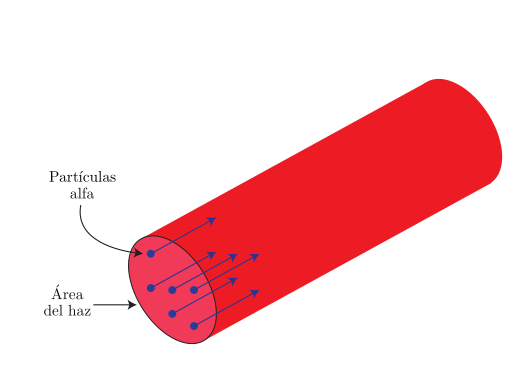
\includegraphics[scale=0.35]{Imagenes/haz.png}
	\caption{Haz de partículas alfa.}
	\label{haz}
\end{figure}

Para cada partícula en la simulación, se considerarán las interacciones que estas tienen con el material del objetivo para determinar la trayectoria que debe seguir al momento de alcanzarlo. Se colocan $10$ detectores que cuenta el paso de partículas alfa con el fin de determinar cuántas de las partículas que inciden en el objetivo se dispersan a un ángulo $\Theta$ respecto de la trayectoria original del haz. Cada detector tiene un área efectiva de $4 cm^2$ y estan dispuestos sobre un círculo centrado en el punto de impacto del haz con el material. Los detectores se encuentran a intervalos de $15^o$ entre $0^o$ y $135^o$ (ver figura \ref{montaje}).
        
\begin{figure}
	\centering
	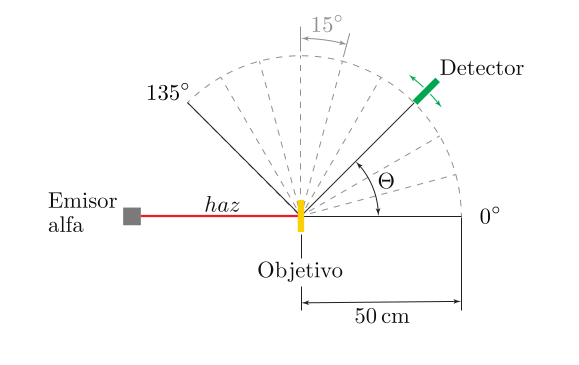
\includegraphics[scale=0.3]{Imagenes/montaje.png}
	\caption{Montaje experimental de la simulación.}     
	\label{montaje}   
\end{figure}
        
        
\section{Resultados}

\begin{table}[H]
	\centering
	\caption{Primera Simulación}
	\begin{tabular}{||c|c||}
	\hline
	\hline
	\multicolumn{2}{||c||}{Run $1$} \\
	\hline
	\hline
	Ángulo del Detector & Mediciones \\
	\hline
	$0^o$   & $28192468$ \\
	$15^o$  & $5202$     \\
	$30^o$  & $295$      \\ 
	$45^o$  & $52$       \\
	$60^o$  & $16$       \\
	$75^o$  & $9$        \\
	$90^o$  & $0$        \\
	$105^o$ & $3$        \\
	$120^o$ & $4$        \\
	$135^o$ & $2$        \\
	\hline
	\hline
	\end{tabular}
\end{table}



\begin{table}[H]
	\centering
	\caption{Segunda Simulación}
	\begin{tabular}{||c|c||}
	\hline
	\hline
	\multicolumn{2}{||c||}{Run $2$} \\
	\hline
	\hline
	Ángulo del Detector & Mediciones \\
	\hline
	$0^o$   & $28194414$ \\
	$15^o$  & $5231$     \\
	$30^o$  & $299$      \\ 
	$45^o$  & $58$       \\
	$60^o$  & $12$       \\
	$75^o$  & $9$        \\
	$90^o$  & $1$        \\
	$105^o$ & $2$        \\
	$120^o$ & $2$        \\
	$135^o$ & $1$        \\
	\hline
	\hline
	\end{tabular}
\end{table}




\begin{table}[H]
	\centering
	\caption{Tercera Simulación}
	\begin{tabular}{||c|c||}
	\hline
	\hline
	\multicolumn{2}{||c||}{Run $3$} \\
	\hline
	\hline
	Ángulo del Detector & Mediciones \\
	\hline
	$0^o$   & $28187047$ \\
	$15^o$  & $5307$     \\
	$30^o$  & $314$      \\ 
	$45^o$  & $60$       \\
	$60^o$  & $18$       \\
	$75^o$  & $11$        \\
	$90^o$  & $5$        \\
	$105^o$ & $3$        \\
	$120^o$ & $0$        \\
	$135^o$ & $3$        \\
	\hline
	\hline
	\end{tabular}
\end{table}





\begin{table}[H]
	\centering
	\caption{Cuarta Simulación}
	\begin{tabular}{||c|c||}
	\hline
	\hline
	\multicolumn{2}{||c||}{Run $4$} \\
	\hline
	\hline
	Ángulo del Detector & Mediciones \\
	\hline
	$0^o$   & $28190247$ \\
	$15^o$  & $5393$     \\
	$30^o$  & $295$      \\ 
	$45^o$  & $46$       \\
	$60^o$  & $26$       \\
	$75^o$  & $11$        \\
	$90^o$  & $6$        \\
	$105^o$ & $1$        \\
	$120^o$ & $1$        \\
	$135^o$ & $1$        \\
	\hline
	\hline
	\end{tabular}
\end{table}




\begin{table}[H]
	\centering
	\caption{Quinta Simulación}
	\begin{tabular}{||c|c||}
	\hline
	\hline
	\multicolumn{2}{||c||}{Run $5$} \\
	\hline
	\hline
	Ángulo del Detector & Mediciones \\
	\hline
	$0^o$   & $28192468$ \\
	$15^o$  & $5202$     \\
	$30^o$  & $295$      \\ 
	$45^o$  & $52$       \\
	$60^o$  & $16$       \\
	$75^o$  & $9$        \\
	$90^o$  & $0$        \\
	$105^o$ & $3$        \\
	$120^o$ & $4$        \\
	$135^o$ & $2$        \\
	\hline
	\hline
	\end{tabular}
\end{table}






\begin{table}[H]
	\centering
	\caption{Sexta Simulación}
	\begin{tabular}{||c|c||}
	\hline
	\hline
	\multicolumn{2}{||c||}{Run $6$} \\
	\hline
	\hline
	Ángulo del Detector & Mediciones \\
	\hline
	$0^o$   & $28192468$ \\
	$15^o$  & $5202$     \\
	$30^o$  & $295$      \\ 
	$45^o$  & $52$       \\
	$60^o$  & $16$       \\
	$75^o$  & $9$        \\
	$90^o$  & $0$        \\
	$105^o$ & $3$        \\
	$120^o$ & $4$        \\
	$135^o$ & $2$        \\
	\hline
	\hline
	\end{tabular}
\end{table}
    
    
    
   
\begin{table}[H]
	\centering
	\caption{Promedio y Desviación Estandar}
	\begin{tabular}{||c|c|c||}
	\hline
	\hline
	Ángulo del Detector & Promedio & Std \\
	\hline
	$0^o$   & $28191519$ & $2557$ \\
	$15^o$  & $5256$     & $78$ \\
	$30^o$  & $299$      & $7$ \\ 
	$45^o$  & $53$       & $5$ \\
	$60^o$  & $17$       & $4$ \\
	$75^o$  & $10$        & $1$ \\
	$90^o$  & $2$        & $3$ \\
	$105^o$ & $2.5$        & $1$ \\
	$120^o$ & $2$        & $1.5$ \\
	$135^o$ & $2$        & $0.75$ \\
	\hline
	\hline
	\end{tabular}
\end{table}
    
    


\begin{figure}[H]
	\centering
	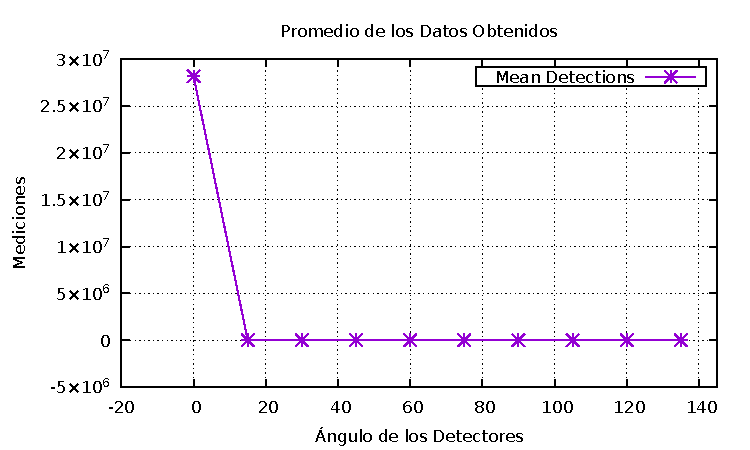
\includegraphics[scale=0.5]{./Codigos/Ajuste.pdf}
	\caption{Ajuste de las medias de los datos obtenidos.}
	\label{ajuste}
\end{figure}



    
    
    
\section{Discusión de Resultados}
\begin{enumerate}
    \item Relacionado con las detecciones de partículas, se desmonta, claramente, el modelo atómico de Thompson. Los datos esperados eran más aleatorios en todas direcciónes luego de pasar a travez de la lámina de oro, cosa que no sucede. Se tiene un $28\%$ de las mediciones a un ángulo llano, cosa que muestra que el átomo está compuesto, en su mayoría, de espacio vacío.
    \item El hecho de que existan pequeñas mediciones a más de $90^o$ significa que existen pequeños pedazos dentro del espacio vacío con una gran concentración de carga que provocan el choque.
    \item El hecho de que solo se tengan mediciones de un $~28\%$ del total de las partículas lanzadas puede deberse a muchos factores, a que el espacio cubierto por los medidores no es tan grande, a que la simulación no toma todas las condisderaciones físicas o, simplemente, $100M$ no es la cantidad adecuada de partículas.
\end{enumerate}



\section{Conclusiones}
\begin{enumerate}
    \item El átomo es en su mayoría espacio vacío y el núcleo es carga positiva confinada.
    \item El modelo planetario del átomo propuesto por Rutherford es, según este experimento, el que mejor modela la realidad.
    \item El software GEANT4 es una gran herramienta para la simulación de eventos en física atómica y de partículas. Y siempre es necesario realizar más simulaciones o iteraciones por simulación para obtener lo más cercano a la realidad.
\end{enumerate}
%\section{Recomendaciones}

\section{Anexos}
%		\begin{figure}[H]
%            \centering
%            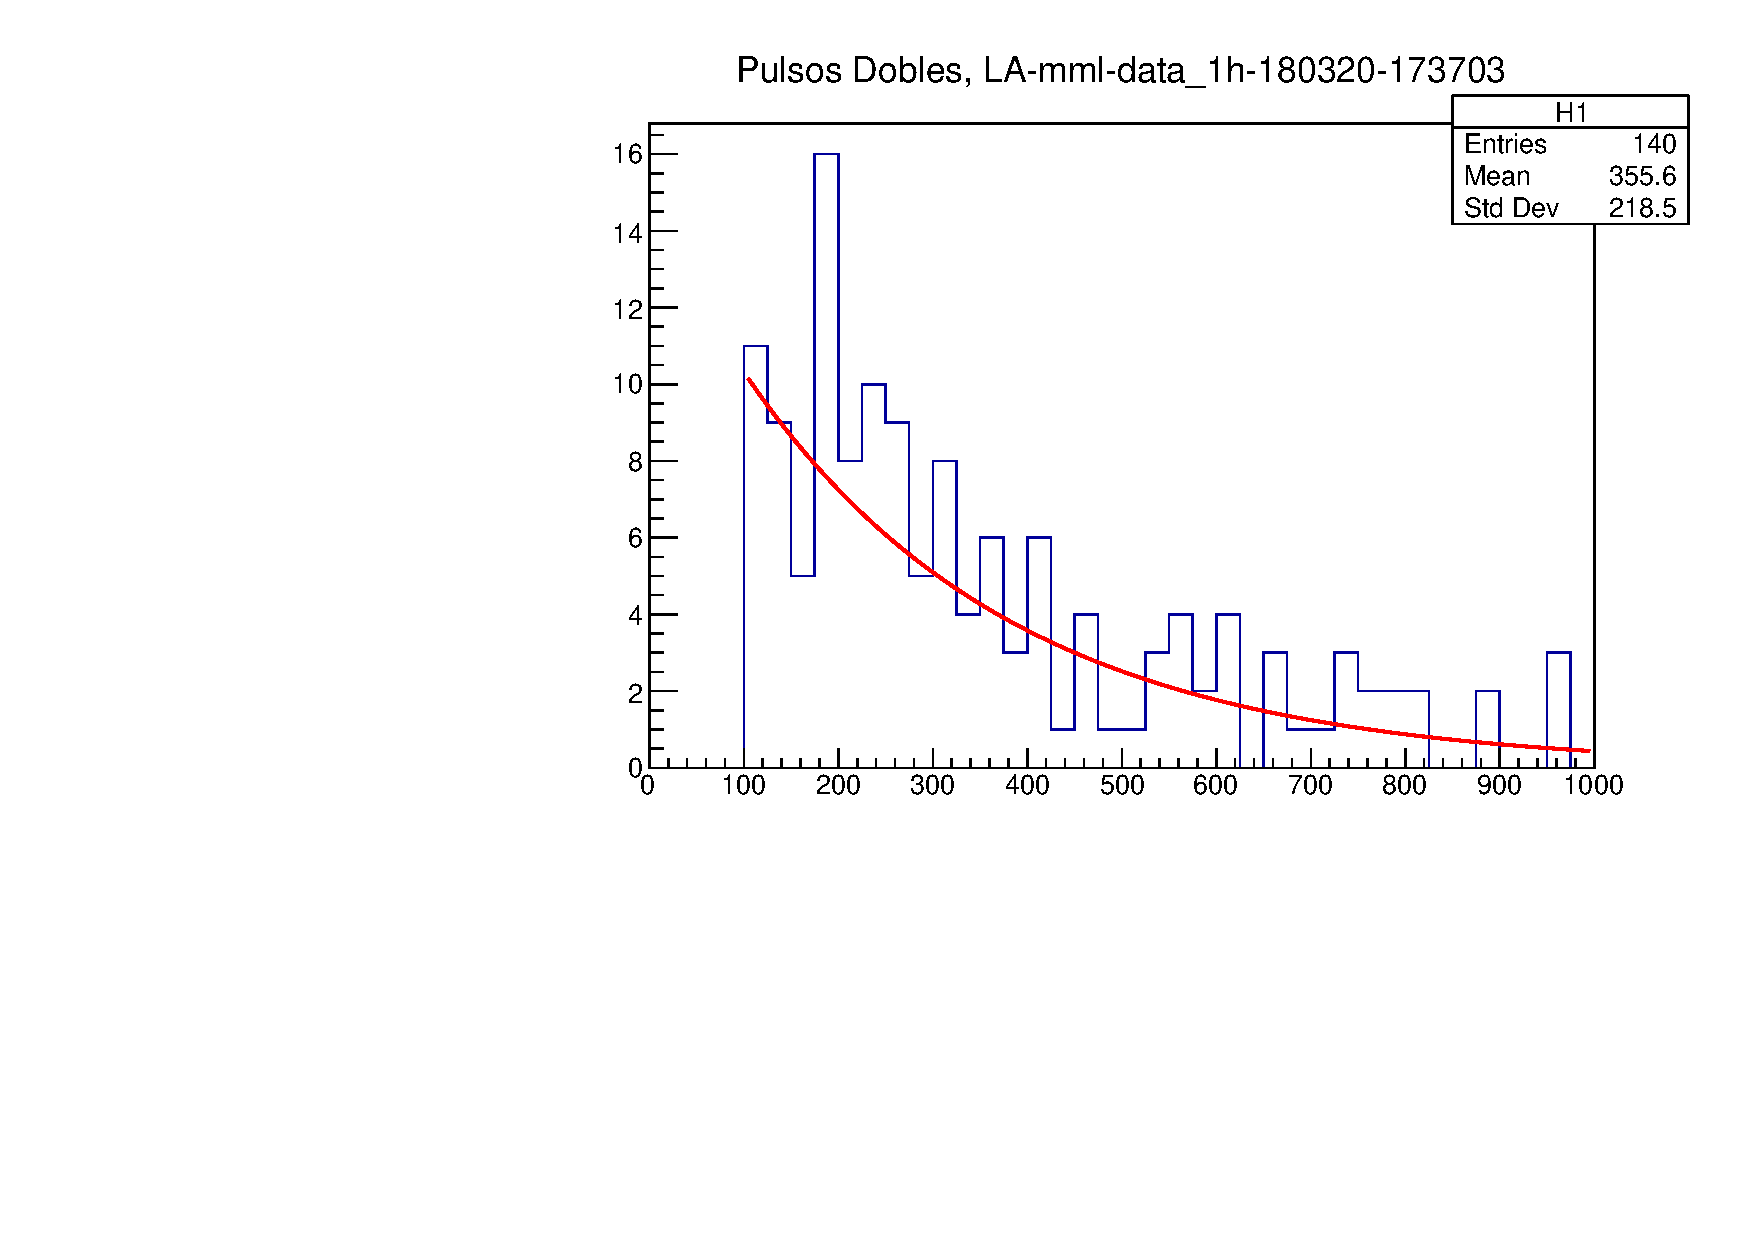
\includegraphics[scale=0.4]{./Imagenes/file1.pdf}
%            \caption{Histograma del archivo de datos terminado en: $173703$}
%            \label{fig:file1}
%        \end{figure}  
%        \begin{figure}[H]
%            \centering
%            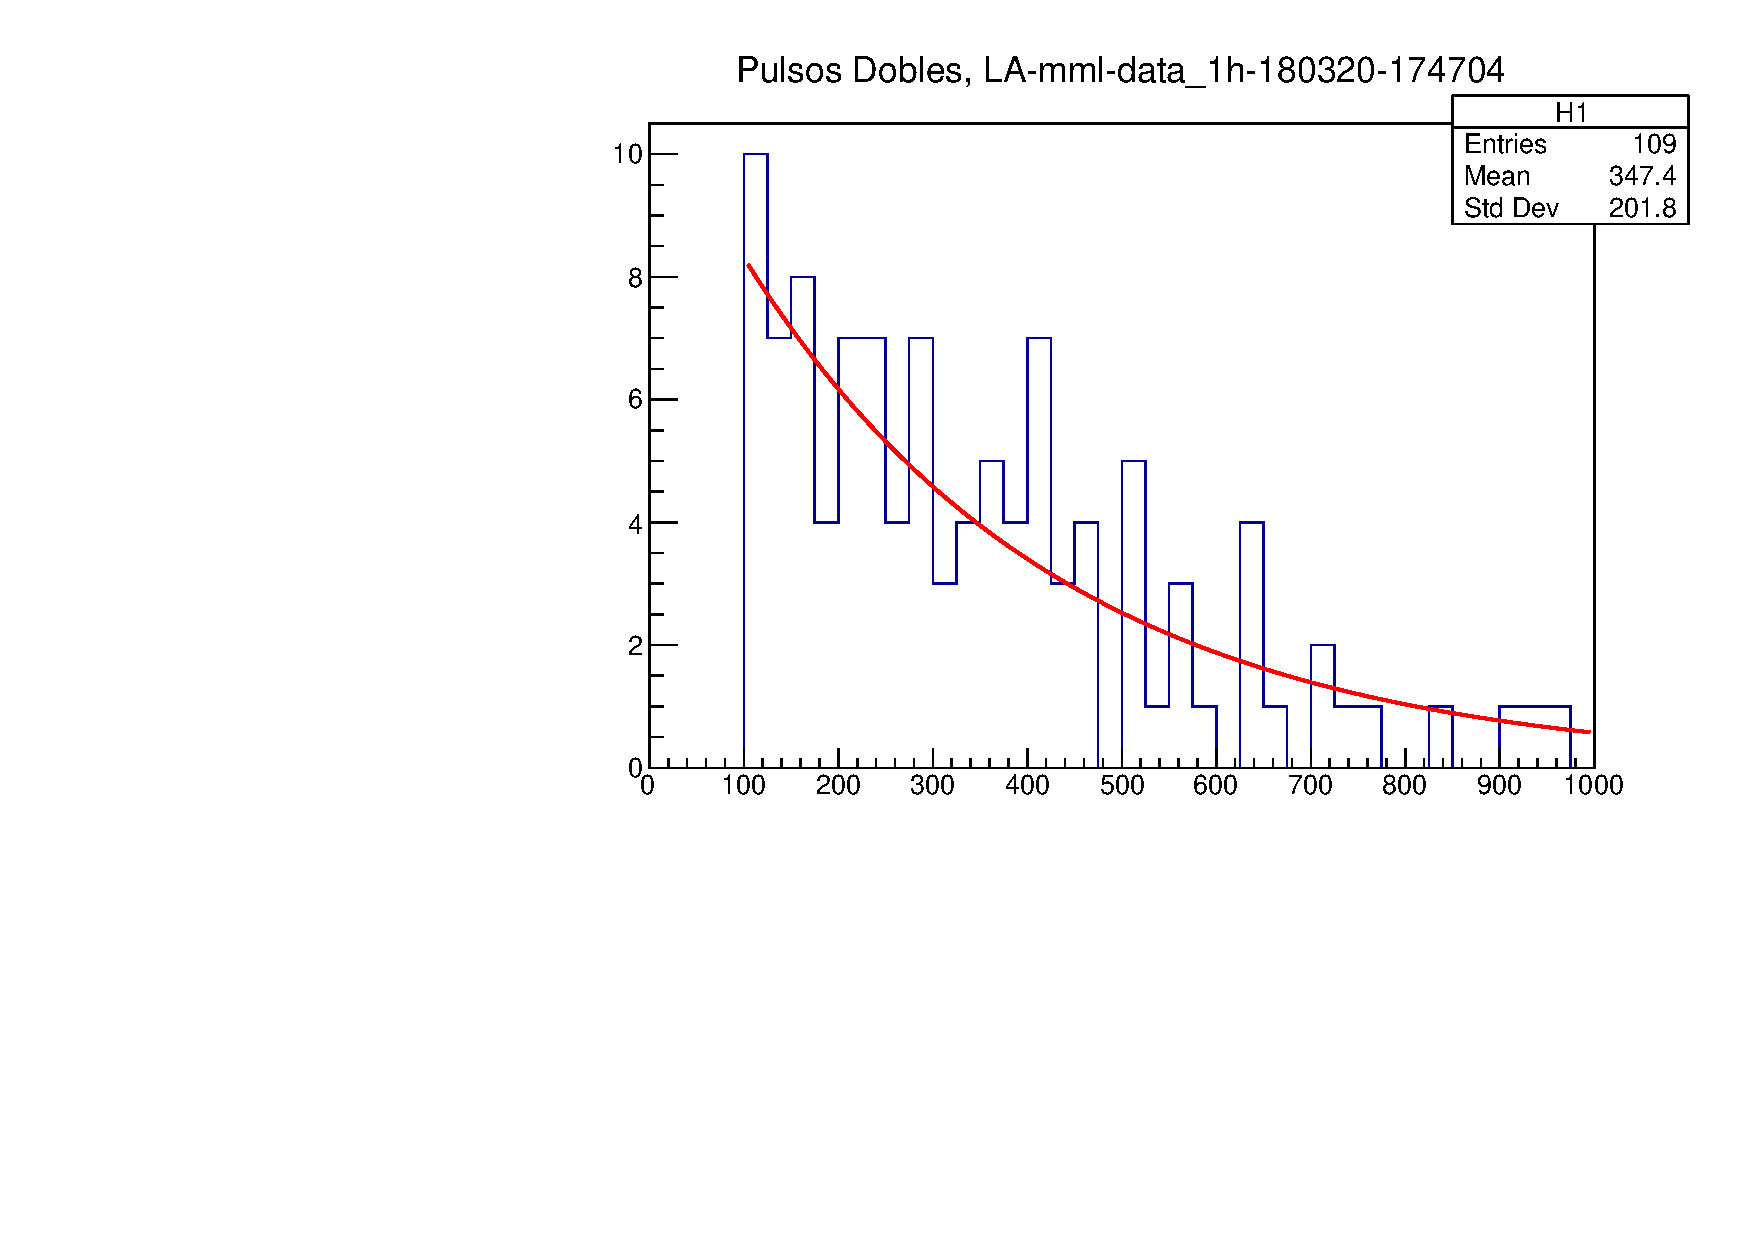
\includegraphics[scale=0.4]{./Imagenes/file2.pdf}
%            \caption{Histograma del archivo de datos terminado en: $174704$}
%            \label{fig:file2}
%        \end{figure} 
%        \begin{figure}[H]
%            \centering
%            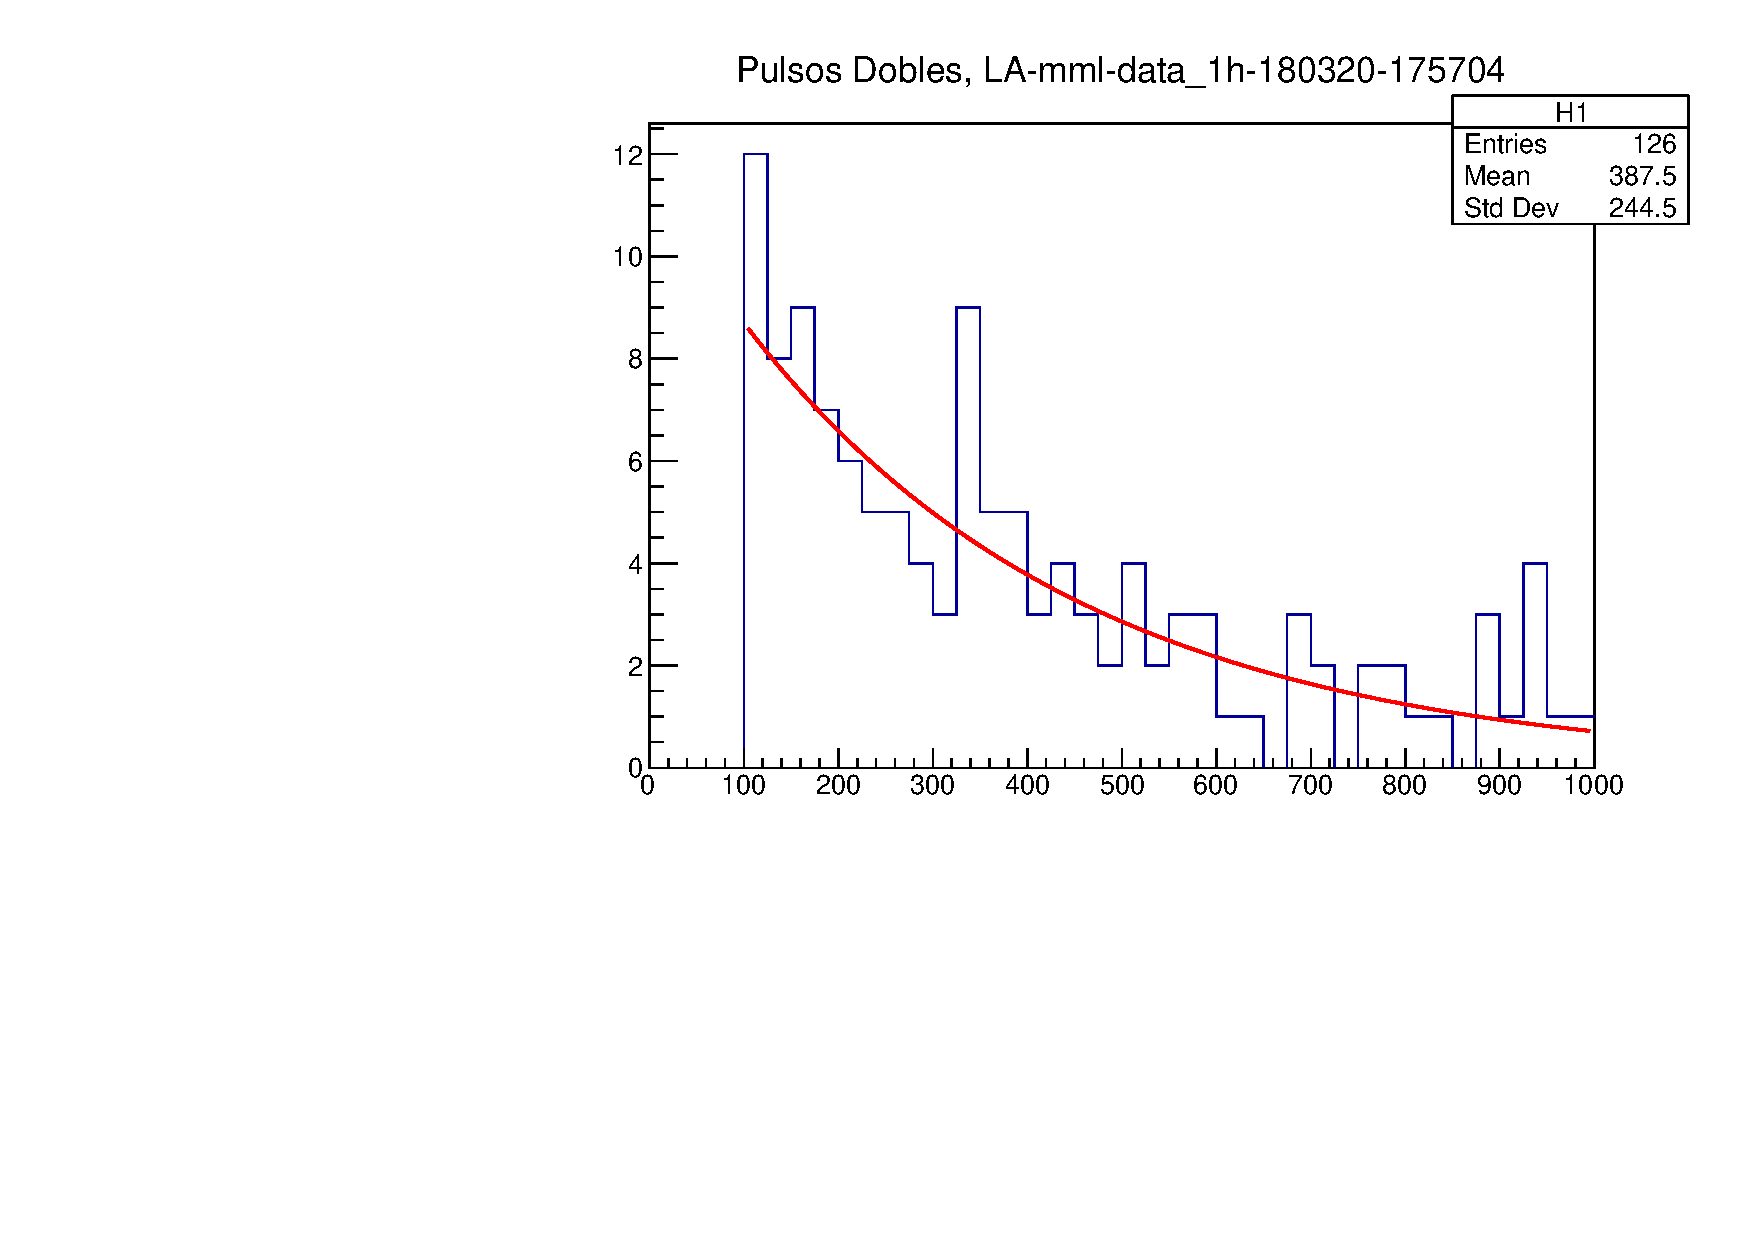
\includegraphics[scale=0.4]{./Imagenes/file3.pdf}
%            \caption{Histograma del archivo de datos terminado en: $175704$}
%            \label{fig:file3}
%        \end{figure}  
%        \begin{figure}[H]
%            \centering
%            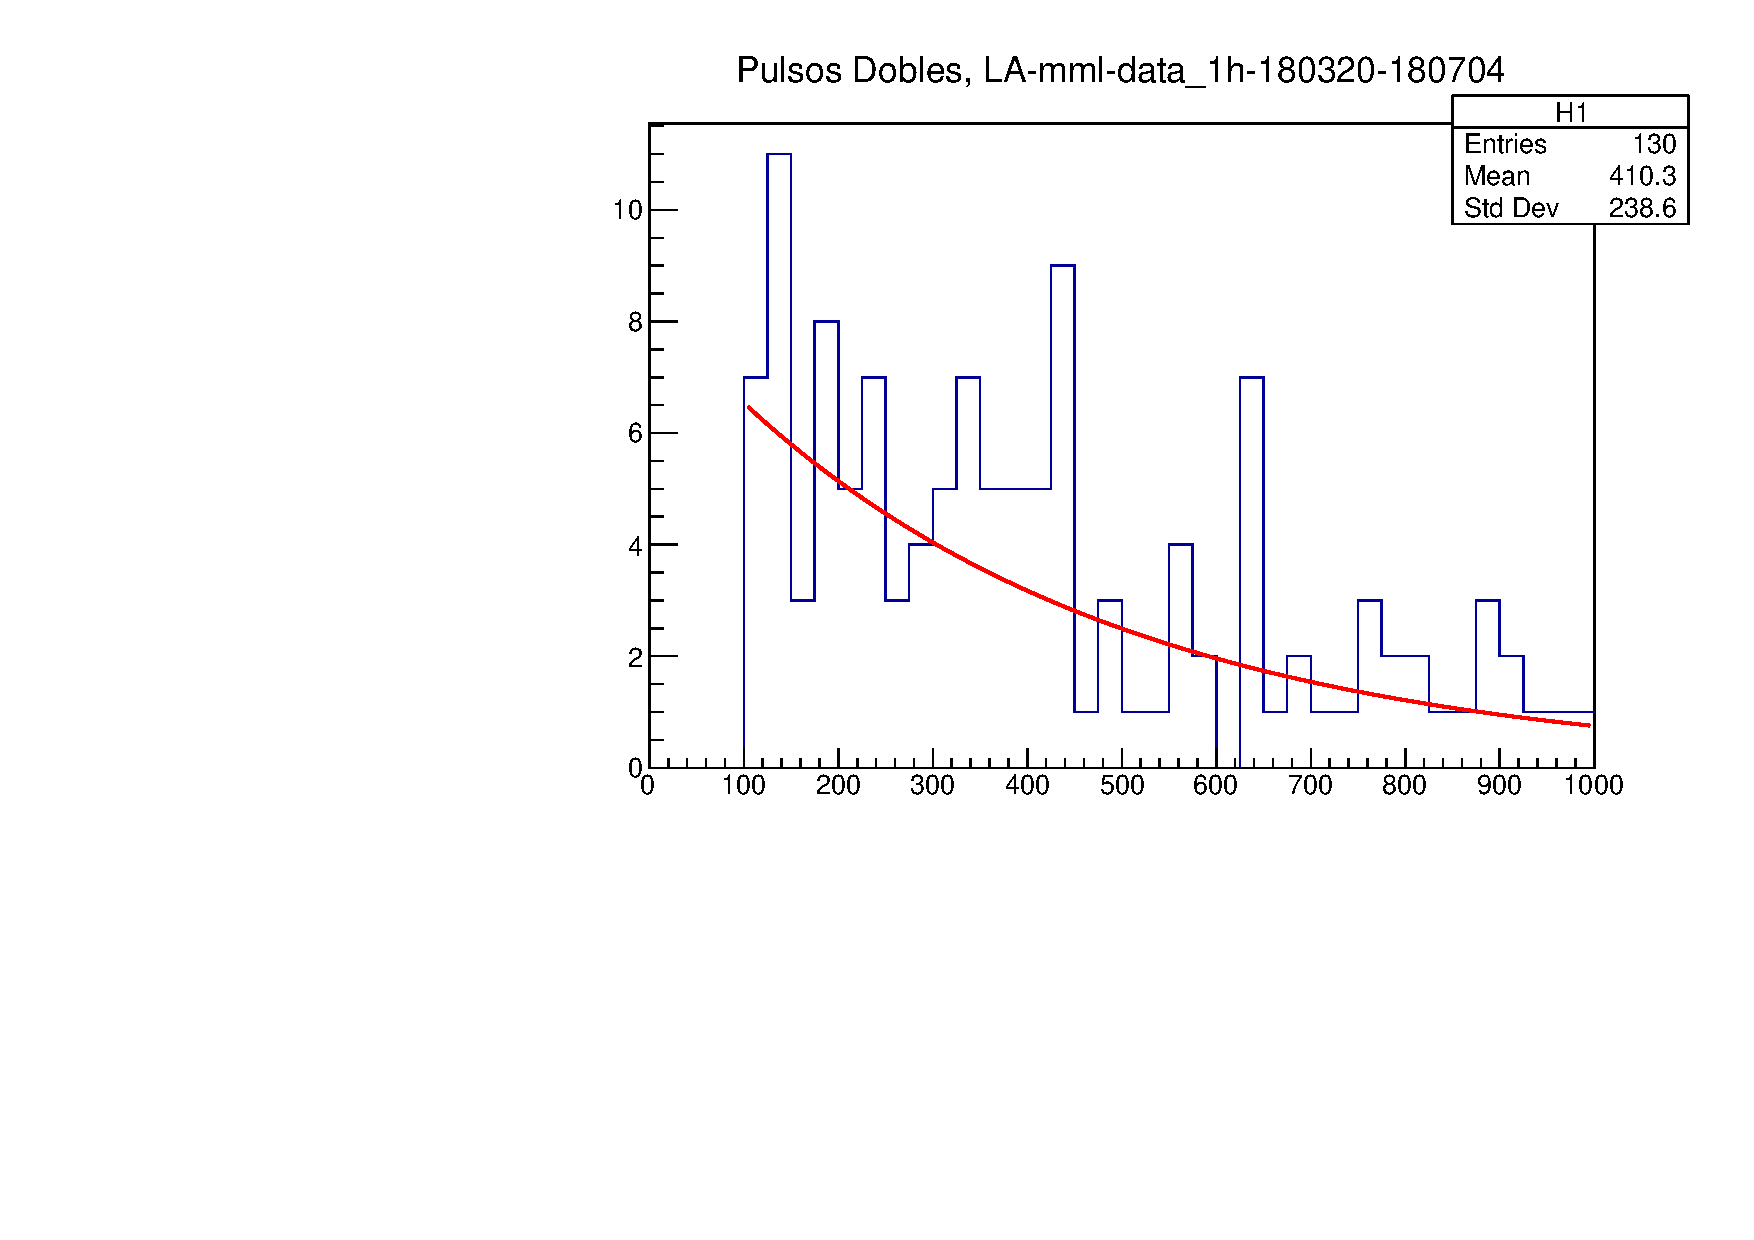
\includegraphics[scale=0.4]{./Imagenes/file4.pdf}
%            \caption{Histograma del archivo de datos terminado en: $180704$}
%            \label{fig:file4}
%         \end{figure} 
%         \begin{figure}[H]
%            \centering
%            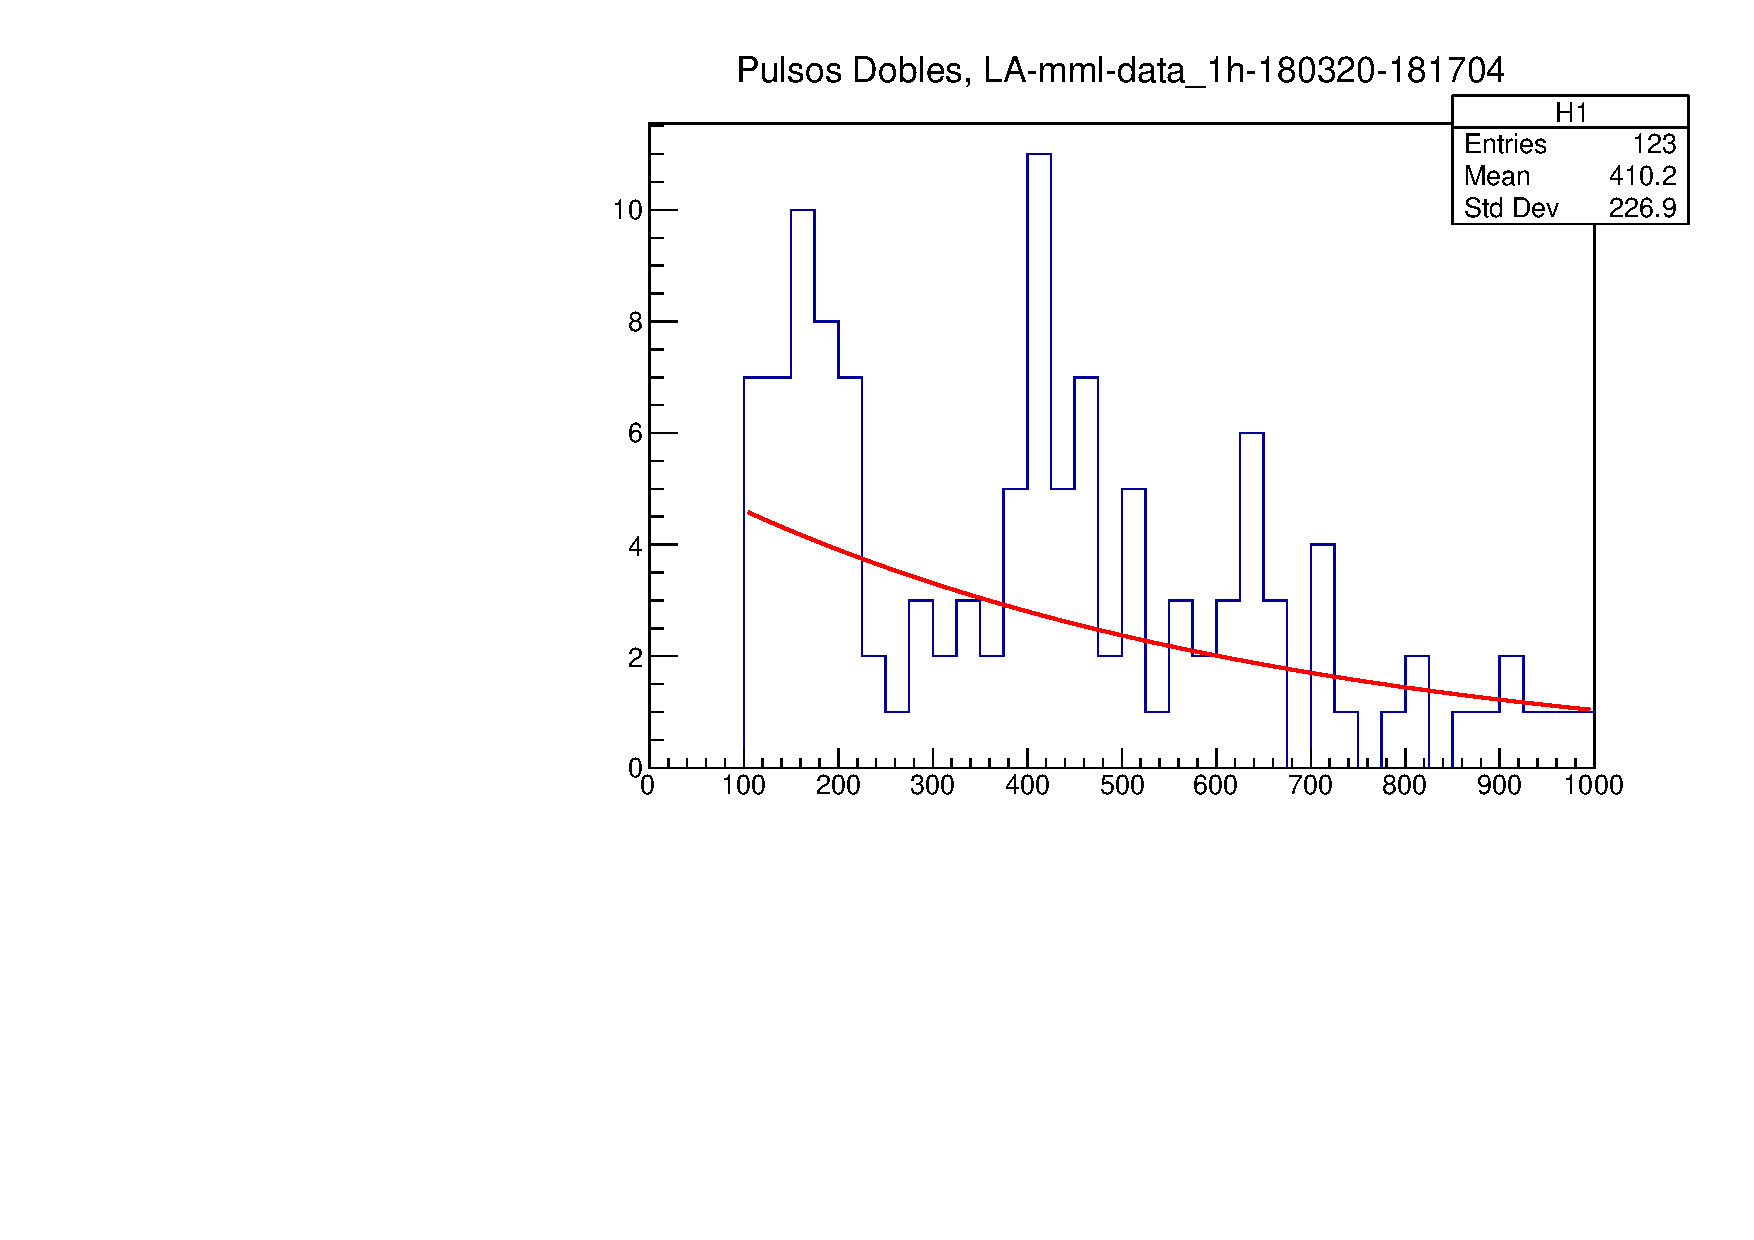
\includegraphics[scale=0.4]{./Imagenes/file5.pdf}
%            \caption{Histograma del archivo de datos terminado en: $181704$}
%            \label{fig:file5}
%         \end{figure} 
%         \begin{figure}[H]
%            \centering
%            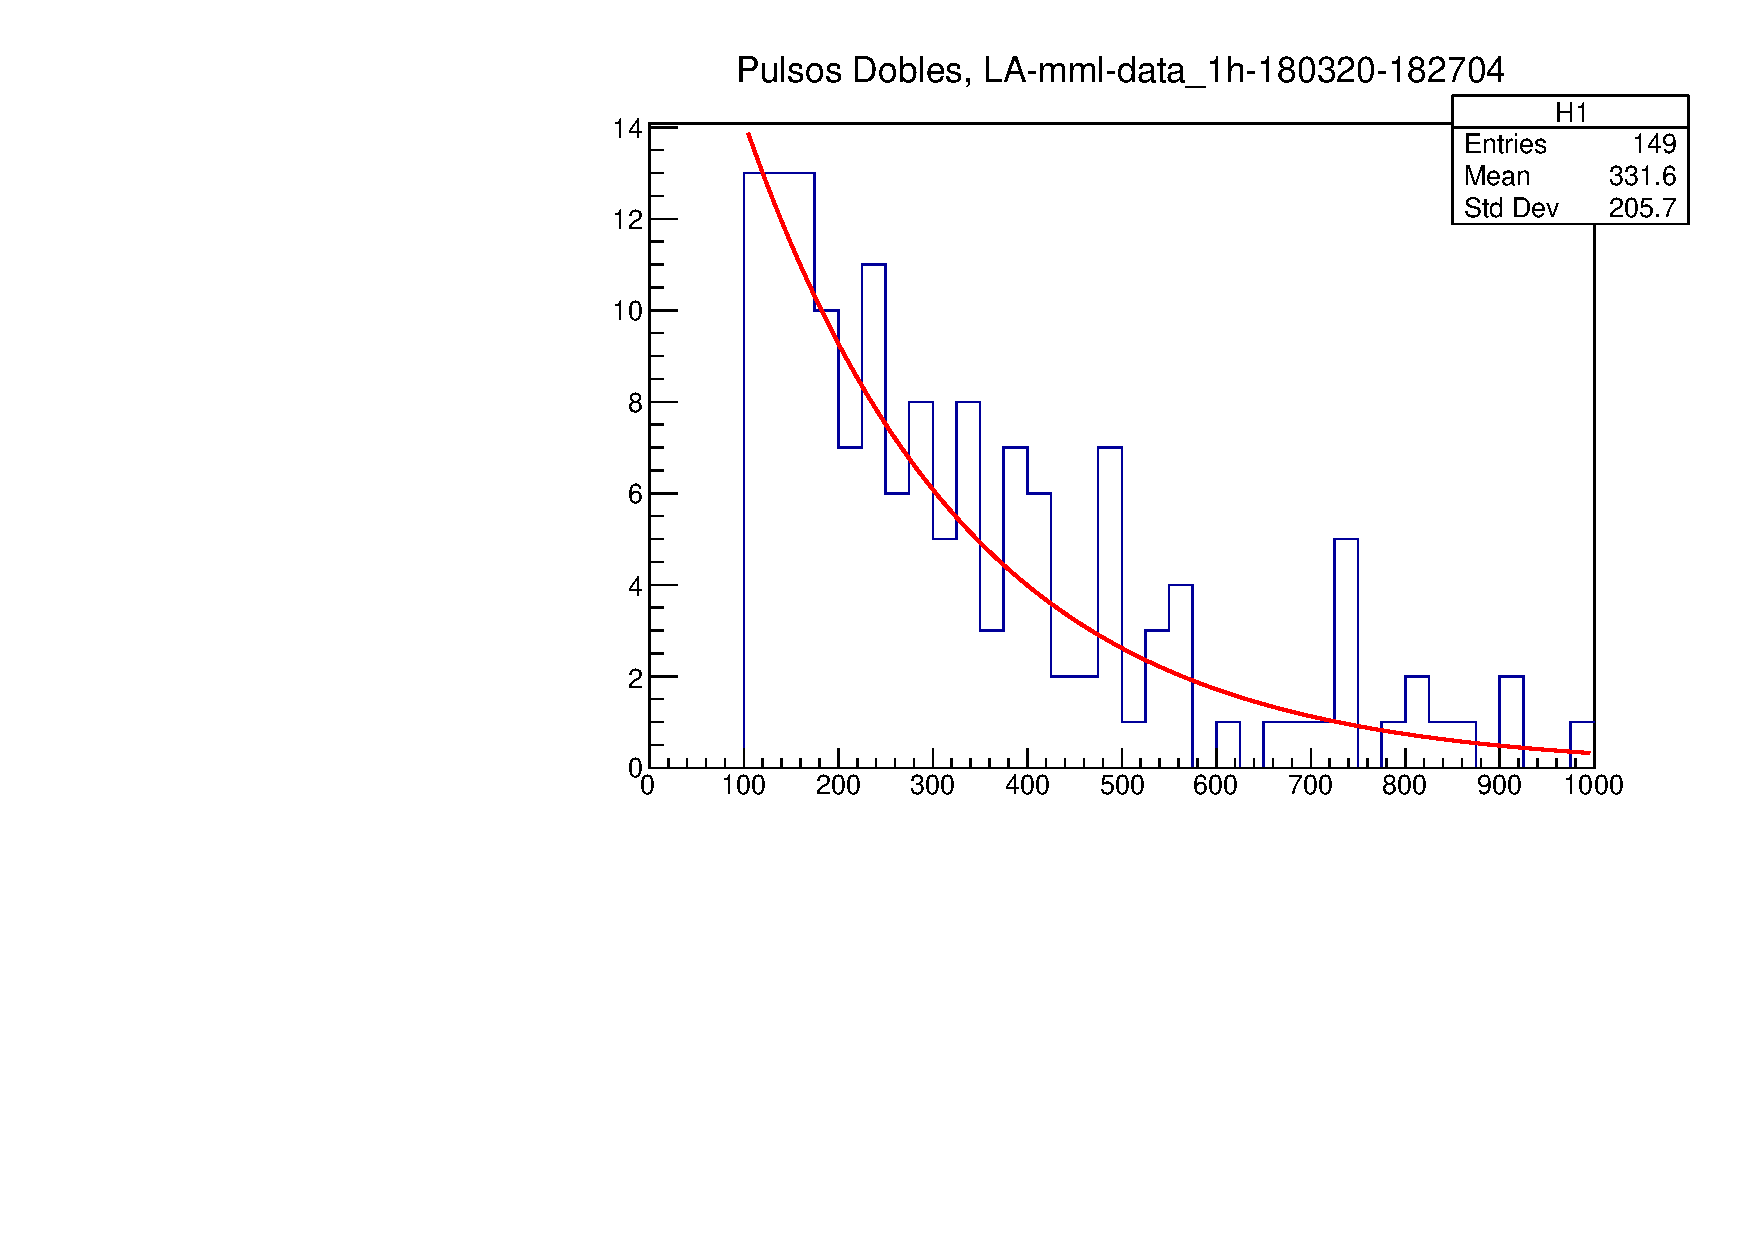
\includegraphics[scale=0.4]{./Imagenes/file6.pdf}
%            \caption{Histograma del archivo de datos terminado en: $182704$}
%            \label{fig:file6}
%         \end{figure} 
        
        
        
        
\begin{thebibliography}{00}
\bibitem{b1} Beiser, A. (1968). \textit{Modern Physics: an introductory survey}. Addison-Wesley Publishing Company.
\bibitem{b2} \textit{Rutherford Scattering} \url{http://hyperphysics.phy-astr.gsu.edu/hbasees/rutsca.html}
\end{thebibliography}

\end{document}


